\subsubsection{Computation of the convolution without FFT}
In the sake of clarity we start with 1D case of convolution.
Suppose we have two functions $f(x)$ and $g(x)$ decomposed in Hermite functions. Their Fourier images will be expressed using the same decomposition coefficients as their real counterparts
but in the basis of $\tilde{\psi}_n(\omega; \lambda), ~~n\in[0,N]$ functions. We can therefore compute their product and project it on the same basis. The coefficients of the product will read:
\begin{equation}
 \hat{fg}_l=\sum_{nm}\hat{f}_n \hat{g}_m T^{nm}_l
\end{equation}
where $T^{nm}_l$ are the following integrals over all space:
\begin{equation}
 T^{nm}_l = \int d\omega_x\omega_y\omega_z~ \tilde{\psi}_n(\omega_x; \lambda)\tilde{\psi}_m(\omega_y; \lambda)\tilde{\psi}_l(\omega_z; \lambda)
\end{equation}
Using the definition of the Hermite functions it is easy to see, that these coefficients can be rewritten in the form:
\begin{eqnarray*}
 T^{ij}_k = (-i)^{i+j+k}\sqrt{\frac{2}{\lambda \sqrt{\pi}}}J_{ijk},\\
 J_{ijk}=\frac{1}{\sqrt{2^{i+j+k} i!j!k!}}\int_{-\infty}^{+\infty}e^{-\frac{3t^2}{2}}H_i(t)H_j(t)H_k(t)
\end{eqnarray*}
The coefficients $J_{ijk}$ are independent of the parameter $\lambda$ and therefore can be computed only once. After computing the Fourier image of
the convolution we can apply the algorithm similar to the one used in section \ref{Sec: HermiteFourierTransition} and obtain values of the convolution 
on the real-space grid.

However the complexity of this approach is $O(N^3)$ and is prohibitive for the applications. One of the way to overcome this hurdle is to decompose 
the tensor $J$ into the tensor products of 1-rank tensors. This decomposition is called canonical polyadic decomposition (CPD) \ref{kruskal1989rank} and is widely used in
psychometry, chemomometrics, signal processing, computer vision and more \ref{kolda2009tensor}. The tensor $J_{ijk}$ is expressed in the following way:
\begin{equation}
 J_{ijk} = \sum_{r=0}^{R} U^{(1)}_{ir} U^{(2)}_{jr} U^{(3)}_{kr} + \epsilon_{ijk}
\end{equation}
The rank $R$ of the decomposition is determined by the relative error of the decomposition. We used Tesor toolbox to perform the calculations \ref{TTB_Software} in the 
case of Hermite decomposition order $N=30$ or equally the size of the tensor $J$ equal to $31$ along each direction.
Figure \ref{pic: CPDError} shows the relative error of the CPD decomposition. We see that the decomposition of the rank $R=44$ is enough to approximate the 
tensor $J$.

\begin{figure}[ht!]
\label{pic: CPDError}
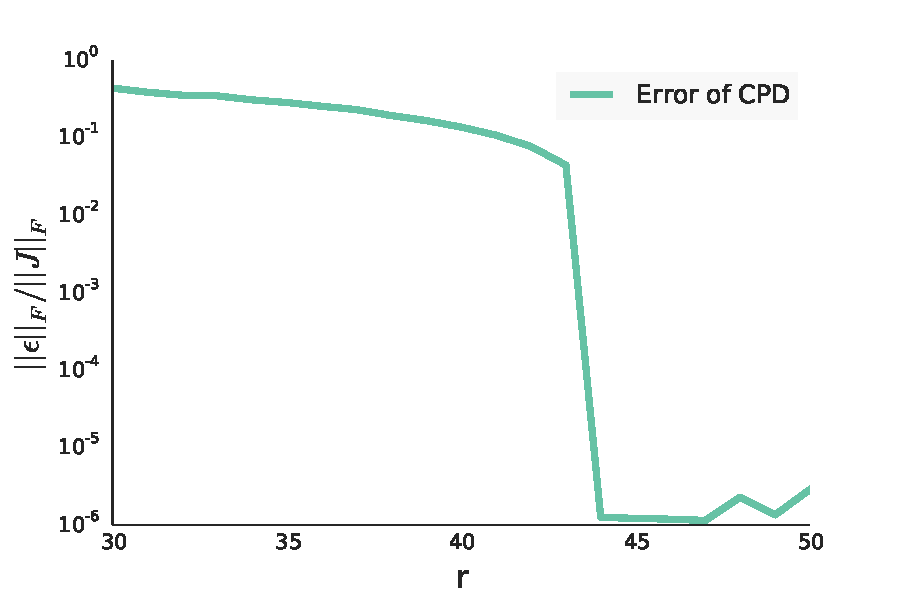
\includegraphics[width=1\textwidth]{Hermite/Fig/CPDError.pdf}
\caption{Relative error of the canonical polyadic decomposition of the tensor $J_{ijk}$ versus the order $r$. 
The size of the tensor $J$ was $31\times 31\times 31$. The relative error was computed using Frobenius norm 
of the residual $\epsilon$ divided by the Frobenius norm of the tesor itself.}
\end{figure}

Therefore the algorithm to compute a convolution in 1D is performed in three steps. First we compute 
\begin{equation}
 \hat{f}'_r=\sum_{n}\hat{f}_n U^{(1)}_{nr};~~
 \hat{g}'_r=\sum_{n}\hat{g}_m U^{(2)}_{mr}
\end{equation}
Then we multiply them together:
\begin{equation}
 \hat{h}'_r=\hat{f}'_r\hat{g}'_r
\end{equation}
And finally we compute the decomposition coefficient of convolution in the Hermite basis:
\begin{equation}
 \hat{h}_l = \sum_{r=0}^{R} \hat{h}'_r U^{(3)}_{lr}
\end{equation}
The complexity of the algorithm therefore becomes $O(2RN + N + RN)$, which is on the scale of $O(N^2)$. Despite the fact that this algorithm has the assympotical
complexity worse than FFT, we believe that it could fit the GPU architecture better than FFT algorithm, because it, unlike FFT,
involves only simple matrix multiplications.